\documentclass[11pt]{article}

\usepackage{amsmath,amsfonts,amssymb,graphicx}
\usepackage[CJKnumber]{xeCJK}
\usepackage{fontspec}
\usepackage[xetex]{hyperref}
\usepackage{xunicode, xltxtra}
\setCJKfamilyfont{tt}{STSong}

% 这里的字体设置是在Mac OS X下的,其它操作系统请修改成对应的字体
% 可以用过fc-list命令查看当前系统所有的字体
\setCJKmainfont[BoldFont=Heiti SC]{STSong} % 中文宋体
\setmainfont{Times New Roman} % 英文Times New Roman

\XeTeXlinebreaklocale "zh"
\widowpenalty=10000
\usepackage{booktabs}
\usepackage{float}
\usepackage{indentfirst}
\usepackage[pagestyles]{titlesec}
\usepackage{titletoc}
\usepackage[top=2cm,bottom=2cm,left=2.5cm,right=1.5cm]{geometry}%全文页面设置:上2cm,下2cm,左2.5cm,右1.5cm。
\usepackage[super,square,numbers]{natbib}
\usepackage{hypernat}
\usepackage{algpseudocode}
\usepackage{algorithm}
\usepackage{tikz}

%行间距和段间距设置
\renewcommand{\paragraph}{\hspace{5pt}}
\titlespacing*{\paragraph}{0em}{0em}{0em}
\linespread{1.25}\selectfont %1.2*1.25=1.5

\makeatletter
\newdimen\bibspace
\setlength\bibspace{0pt}
\renewenvironment{thebibliography}[1]{
  \bibfont\bibsection\parindent \z@\list
  {\@biblabel{\arabic{NAT@ctr}}}{\@bibsetup{#1}
    \setcounter{NAT@ctr}{0}}
  \ifNAT@openbib
  \renewcommand\newblock{\par}
  \else
  \renewcommand\newblock{\hskip .11em \@plus.33em \@minus.07em}
  \fi
  \sloppy\clubpenalty4000\widowpenalty4000
  \sfcode`\.=1000\relax
  \let\citeN\cite \let\shortcite\cite
  \let\citeasnoun\cite
  \itemsep\bibspace
  \parsep\z@skip 
}{\def\@noitemerr{
    \PackageWarning{natbib}
    {Empty `thebibliography' environment}}
  \endlist\vskip-\lastskip
}

\def\enumerate{
  \ifnum \@enumdepth >\thr@@\@toodeep\else
  \advance\@enumdepth\@ne
  \edef\@enumctr{enum\romannumeral\the\@enumdepth}
  \expandafter
  \list
  \csname label\@enumctr\endcsname
  {\usecounter\@enumctr\def\makelabel##1{\hss\llap{##1}}
    \addtolength{\parsep}{-5pt}
    \addtolength{\topsep}{-5pt}
  }
  \fi}

\def\itemize{
  \ifnum \@itemdepth >\thr@@\@toodeep\else
  \advance\@itemdepth\@ne
  \edef\@itemitem{labelitem\romannumeral\the\@itemdepth}
  \expandafter
  \list
  \csname\@itemitem\endcsname
  {\def\makelabel##1{\hss\llap{##1}}
    \addtolength{\parsep}{-5pt}
    \addtolength{\topsep}{-5pt}
  }
  \fi}

\renewenvironment{description}
{\list{}{\labelwidth\z@ \itemindent-\leftmargin
    \let\makelabel\descriptionlabel
    \addtolength{\parsep}{-5pt}
    \addtolength{\itemindent}{10pt}
    \addtolength{\topsep}{-5pt}
  }
}
{\endlist}
\makeatother

%兼容Word字号
\newcommand{\chuhao}{\fontsize{42pt}{\baselineskip}\selectfont}     % 初号
\newcommand{\xiaochuhao}{\fontsize{36pt}{\baselineskip}\selectfont} % 小初号
\newcommand{\yichu}{\fontsize{32pt}{\baselineskip}\selectfont}      % 一初号
\newcommand{\yihao}{\fontsize{28pt}{\baselineskip}\selectfont}      % 一号
\newcommand{\erhao}{\fontsize{21pt}{\baselineskip}\selectfont}      % 二号
\newcommand{\xiaoerhao}{\fontsize{18pt}{\baselineskip}\selectfont}  % 小二号
\newcommand{\sanhao}{\fontsize{15.75pt}{\baselineskip}\selectfont}  % 三号
\newcommand{\xiaosanhao}{\fontsize{15pt}{\baselineskip}\selectfont}  % 小三号
\newcommand{\sihao}{\fontsize{14pt}{\baselineskip}\selectfont}      % 四号
\newcommand{\xiaosihao}{\fontsize{12pt}{\baselineskip}\selectfont}  % 小四号
\newcommand{\wuhao}{\fontsize{10.5pt}{\baselineskip}\selectfont}    % 五号
\newcommand{\xiaowuhao}{\fontsize{9pt}{\baselineskip}\selectfont}   % 小五号
\newcommand{\liuhao}{\fontsize{7.875pt}{\baselineskip}\selectfont}  % 六号
\newcommand{\qihao}{\fontsize{5.25pt}{\baselineskip}\selectfont}    % 七号

\newenvironment{sudaequation}{\begin{equation}\wuhao}{\end{equation}}

\renewcommand\refname{参考文献}
\renewcommand\tablename{表}
\renewcommand\figurename{图}
\floatname{algorithm}{算法}

\renewcommand{\thetable}{\arabic{section}.\arabic{table}}
\renewcommand{\theequation}{式\arabic{section}.\arabic{equation}}
\renewcommand{\thefigure}{\arabic{section}.\arabic{figure}}
\renewcommand{\thealgorithm}{\arabic{section}.\arabic{algorithm}}


%在pdf元数据中保存作者等信息
\hypersetup{
  pdfauthor = 王烨,
  pdftitle = 基于身份的即时消息安全系统设计与实现,
  pdfsubject = 基于身份的即时消息安全系统设计与实现,
  pdfkeywords = 基于身份加密 即时消息 iOS安全,
  colorlinks = true,
  linkcolor = black,
  citecolor = black,
  urlcolor = blue
}

%页眉页脚设置
\newpagestyle{main}{
  \sethead{}{\xiaowuhao{苏州大学本科生毕业设计(论文)}}{}
  \setfoot{}{\thepage}{}\headrule
}

%一级标题小二号宋体加粗
%二级标题小三号宋体加粗
\titleformat{\section}{\centering\xiaoerhao\bfseries}{\thesection}{0.2em}{}
\titleformat{\subsection}{\raggedright\xiaosanhao\bfseries}{\thesubsection}{0.1em}{}
\titleformat{\subsubsection}{\raggedright\xiaosihao\bfseries}{\thesubsubsection}{0.1em}{}

%设置中文的一级标题
%并将二级标题恢复为阿拉伯数字
\renewcommand{\thesection}{第\CJKnumber{\arabic{section}}章} 
\renewcommand{\thesubsection}{\arabic{section}.\arabic{subsection}}

%文档开始
\begin{document}
%目录等采用罗马数字页码
\pagenumbering{Roman}

\pagestyle{main}

%设置目录格式
\titlecontents{section}[0pt]{\addvspace{2pt}\filright\bfseries\sihao}{\contentspush{\thecontentslabel\
  }}{}{\textnormal{\titlerule*[8pt]{.}\contentspage}}
\titlecontents{subsection}[2em]{\addvspace{2pt}\filright\sihao}{\contentspush{\thecontentslabel\
  }}{}{\titlerule*[8pt]{.}\contentspage}
\titlecontents{subsubsection}[4em]{\addvspace{2pt}\filright\sihao}{\contentspush{\thecontentslabel\
  }}{}{\titlerule*[8pt]{.}\contentspage}
\renewcommand{\contentsname}{目录}
\tableofcontents

\newpage
%正文小四号宋体
\xiaosihao

%中英文摘要
\begin{center}
  \xiaoerhao{\textbf{摘\hspace{1em}要}}
\end{center}

\paragraph
苏大本科生论文{\LaTeX}模板

\vspace{2em}
\leftline{\textbf{关键词:}苏大;论文;模板}

\newpage
\begin{center}
  \xiaoerhao{\textbf{Abstract}}
\end{center}

\paragraph
Soochow university undergraduate thesis {\LaTeX} template

\vspace{2em}
\leftline{\textbf{Keywords:} Soochow university; thesis; template}


\newpage
%正文使用阿拉伯数字页码
\pagenumbering{arabic}
\setcounter{page}{1}
%前言
\section*{前言}
\addcontentsline{toc}{section}{前言}
\paragraph
前言内容。。。


%第一章开始
\newpage
\section{绪论}
\label{section1}
\paragraph
本章首先介绍了本文的研究背景和意义,随后简要介绍了。。。

\subsection{研究背景及意义}
\paragraph
这是研究背景及意义。

\subsection{XXXX简介}
\paragraph
这里是简介

\subsection{主要工作及创新点}
\paragraph
本文主要工作及创新点如下:
\begin{enumerate}
  \item 第一点。
  \item 第二点。
  \item 。。。
\end{enumerate}

\subsection{本文组织结构}
\paragraph
本文分为六章,各章内容安排如下:

\paragraph
\ref{section1}:绪论,介绍本文的研究背景和意义。。。



%第二章
\newpage
%重置各种计数器(图、表格和算法)
\setcounter{table}{0}
\setcounter{figure}{0}
\setcounter{algorithm}{0}
\section{公式和伪代码}
\label{chapter2}
\paragraph
这是第二章。。。

\subsection{插入公式}
下面是一个公式:
\begin{sudaequation}
(g',g,g^{\alpha},g^{(\alpha^2)},\ldots,g^{(\alpha^q)},g^{(\alpha^{q+2})},\ldots,g^{(\alpha^{2q})})\in G^{2q+1}
\end{sudaequation}
公式也可以写在文字中:$g_1=g^\alpha \in G$。

\subsection{插入伪代码}
\paragraph
下面的伪代码描述了一个算法:
\begin{algorithm}[H]
\caption{算法甲}\label{somealgorithm}
\begin{algorithmic}[1]
\Procedure{someAlgorithm}{}
   \State $\alpha \gets random()$
   \State $g \gets random()$
   \State $h \gets random()$
   \State $g_1 \gets g^\alpha$
  \State \textbf{return} $(\alpha ,g,g_1,h)$\Comment{这里写注释}
\EndProcedure
\end{algorithmic}
\end{algorithm}


\newpage
\setcounter{table}{0}
\setcounter{figure}{0}
\setcounter{algorithm}{0}
\section{如何插入表格}
\label{chapter3}
\paragraph
这是第三章。。。。。。。。。

\subsection{插入表格}
\paragraph
可以用下面的办法插入表格:

\begin{table}[H]
  \begin{center}
    \caption{表格的标题}
    \begin{tabular}{|c|l|}
      \hline
      第一行1 & 第一行2 \\
      \hline
      第二行1 & 第二行2 \\
      \hline
    \end{tabular}
  \end{center}
\end{table}

\subsection{插入较为复杂的表格}

下面是一个稍微复杂一些的表格:
\begin{table}[H]
  \begin{center}
    \caption{复杂的表格标题}
    \begin{tabular}{|p{0.33\textwidth}|p{0.24\textwidth}|p{0.21\textwidth}|}
      \hline
      第一行1 & 第一行2 & 第一行3 \\
      \hline
      第二行1 & \multicolumn{2}{|l|}{第二行合并单元格} \\
      \hline
    \end{tabular}
  \end{center}
\end{table}


\newpage
\setcounter{table}{0}
\setcounter{figure}{0}
\section{如何插图}
\label{chapter4}
\paragraph
{\LaTeX}里面可以插入各种图形。

\subsection{插入PNG格式}
\paragraph
便携式网络图形(Portable Network Graphics,PNG)是一种无损压缩的位图图形格式,支持索引、灰度、RGB[A]三种颜色方案以及Alpha通道等特性。

\begin{figure}[H]
\centering
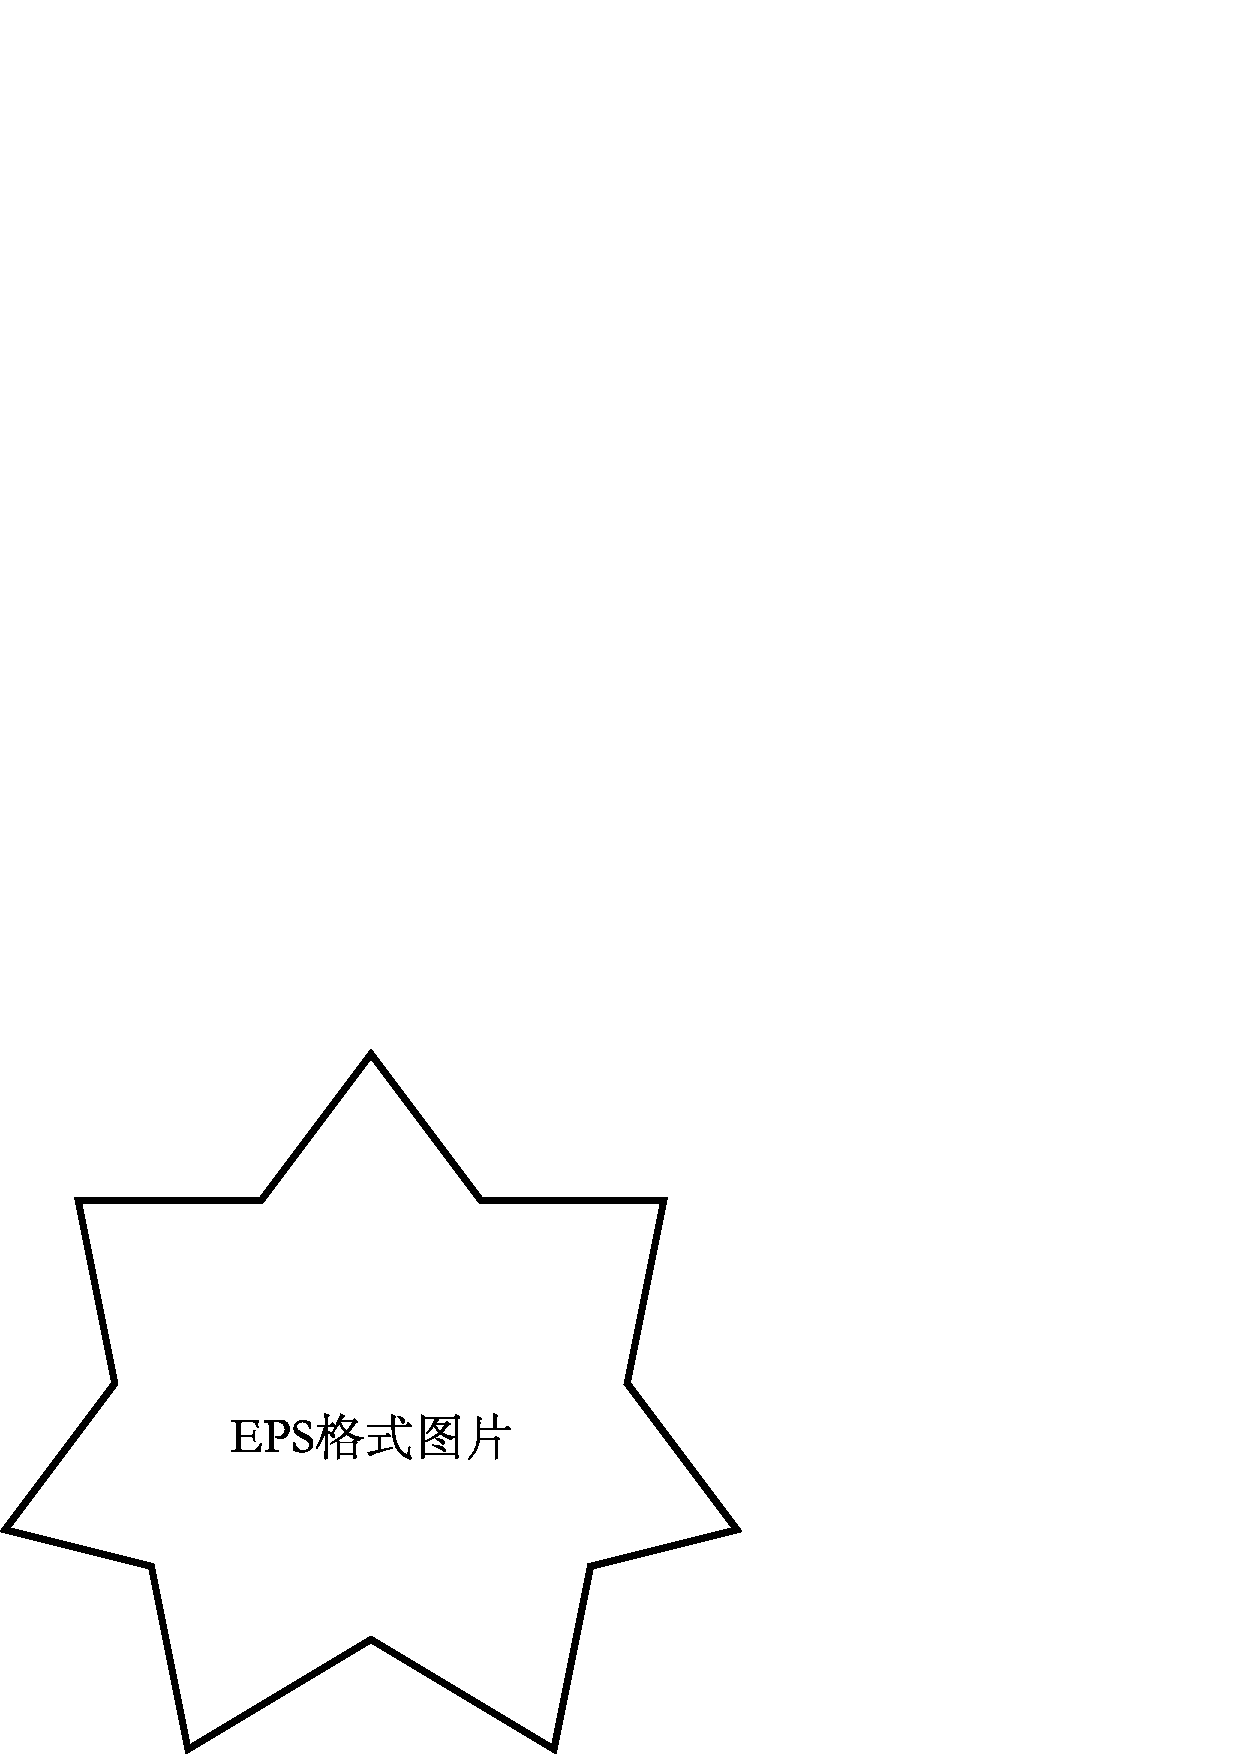
\includegraphics[scale=0.6]{images/pic.png}
\caption{PNG格式图片}
\end{figure}

\subsection{插入EPS格式}
\paragraph
EPS(英文全称:Encapsulated PostScript)是PostScript的一种延伸类型。

\begin{figure}[H]
\centering
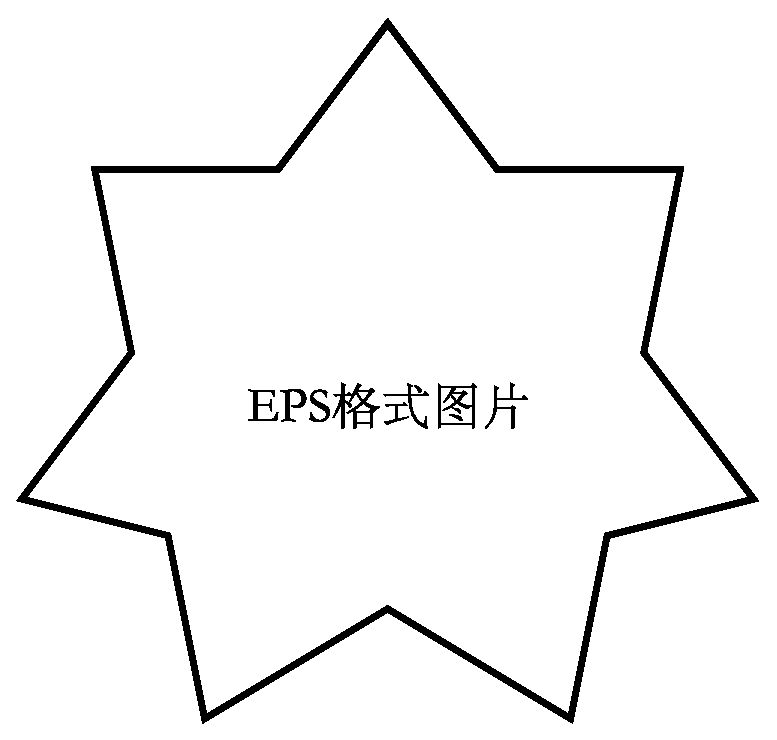
\includegraphics[scale=0.6]{images/pic.eps}
\caption{EPS格式图片}
\end{figure}

\subsection{插入PGF宏}
\paragraph
PGF是一种可以画出矢量图形的语言。

\begin{figure}[H]
\centering
\scalebox{1.2}{% Graphic for TeX using PGF
% Title: /Users/wang/Desktop/pic.dia
% Creator: Dia v0.97.2
% CreationDate: Fri May 11 17:26:22 2012
% For: wang
% \usepackage{tikz}
% The following commands are not supported in PSTricks at present
% We define them conditionally, so when they are implemented,
% this pgf file will use them.
\ifx\du\undefined
  \newlength{\du}
\fi
\setlength{\du}{15\unitlength}
\begin{tikzpicture}
\pgftransformxscale{1.000000}
\pgftransformyscale{-1.000000}
\definecolor{dialinecolor}{rgb}{0.000000, 0.000000, 0.000000}
\pgfsetstrokecolor{dialinecolor}
\definecolor{dialinecolor}{rgb}{1.000000, 1.000000, 1.000000}
\pgfsetfillcolor{dialinecolor}
\pgfsetlinewidth{0.100000\du}
\pgfsetdash{}{0pt}
\pgfsetdash{}{0pt}
\pgfsetbuttcap
\pgfsetmiterjoin
\pgfsetlinewidth{0.100000\du}
\pgfsetbuttcap
\pgfsetmiterjoin
\pgfsetdash{}{0pt}
\definecolor{dialinecolor}{rgb}{1.000000, 1.000000, 1.000000}
\pgfsetfillcolor{dialinecolor}
\fill (25.394079\du,6.850000\du)--(27.253092\du,9.328684\du)--(30.351447\du,9.328684\du)--(29.731776\du,12.427039\du)--(31.590789\du,14.905724\du)--(29.112105\du,15.525395\du)--(28.492434\du,18.623750\du)--(25.394079\du,16.764737\du)--(22.295724\du,18.623750\du)--(21.676053\du,15.525395\du)--(19.197368\du,14.905724\du)--(21.056382\du,12.427039\du)--(20.436711\du,9.328684\du)--(23.535066\du,9.328684\du)--cycle;
\definecolor{dialinecolor}{rgb}{0.000000, 0.000000, 0.000000}
\pgfsetstrokecolor{dialinecolor}
\draw (25.394079\du,6.850000\du)--(27.253092\du,9.328684\du)--(30.351447\du,9.328684\du)--(29.731776\du,12.427039\du)--(31.590789\du,14.905724\du)--(29.112105\du,15.525395\du)--(28.492434\du,18.623750\du)--(25.394079\du,16.764737\du)--(22.295724\du,18.623750\du)--(21.676053\du,15.525395\du)--(19.197368\du,14.905724\du)--(21.056382\du,12.427039\du)--(20.436711\du,9.328684\du)--(23.535066\du,9.328684\du)--cycle;
\pgfsetbuttcap
\pgfsetmiterjoin
\pgfsetdash{}{0pt}
\definecolor{dialinecolor}{rgb}{0.000000, 0.000000, 0.000000}
\pgfsetstrokecolor{dialinecolor}
\draw (25.394079\du,6.850000\du)--(27.253092\du,9.328684\du)--(30.351447\du,9.328684\du)--(29.731776\du,12.427039\du)--(31.590789\du,14.905724\du)--(29.112105\du,15.525395\du)--(28.492434\du,18.623750\du)--(25.394079\du,16.764737\du)--(22.295724\du,18.623750\du)--(21.676053\du,15.525395\du)--(19.197368\du,14.905724\du)--(21.056382\du,12.427039\du)--(20.436711\du,9.328684\du)--(23.535066\du,9.328684\du)--cycle;
% setfont left to latex
\definecolor{dialinecolor}{rgb}{0.000000, 0.000000, 0.000000}
\pgfsetstrokecolor{dialinecolor}
\node at (25.428505\du,13.616495\du){PGF宏};
\end{tikzpicture}
}
\caption{PGF宏}
\end{figure}


\newpage
\setcounter{table}{0}
\setcounter{figure}{0}
\setcounter{algorithm}{0}
\input{sections/chapter_5.tex}

\newpage
\setcounter{table}{0}
\setcounter{figure}{0}
\setcounter{algorithm}{0}
\section{总结}
\label{chapter6}

\subsection{本文总结}
\paragraph
本文总结。。。

\subsection{后续工作展望}
\paragraph
后续展望。。。


\newpage
\addcontentsline{toc}{section}{参考文献}
\bibliographystyle{sudaunsrt} %设置参考文献样式
\bibliography{references} %参考文献数据库为references.bib

\newpage
\input{sections/acknowledgements.tex}

\newpage
\section*{附录}
\addcontentsline{toc}{section}{附录}
本论文撰写过程中所使用的软件简介

\begin{description}
  \item[Emacs] 强大的文本编辑器。
  \item[TeX Live] 一个广泛应用的跨平台{\TeX}发行套件。
  \item[make] 自动编译文档。
\end{description}


\end{document}
